\chapter{Konzeption und Realisierung}
\label{ch:04_konzeption_realisierung}

Im folgenden Kapitel wird der Aufbau und die technische Umsetzung des in C++ und OpenGL
implementierten Test-Frameworks \ac{HyDra} beschrieben.
Es werden die Struktur der Daten, die Implementierungen der untersuchten Rendering-Pipelines, die Implementierungen der
verwendeten \ac{NPR}-Effekte, die individuellen architektonischen Limitationen sowie die Umsetzung der
Leistungsmessungskomponenten erläutert.
Das implementierte Programm fungiert als Untersuchungs- und Messinstrument, das eine Sandbox-Umgebung bereitstellt, in
der das Verhalten der verschiedenen Rendering-Pipelines erprobt werden kann.

Der Aufbau des \ac{HyDra} Frameworks folgt im Wesentlichen den Kernparadigmen der maximalen Vergleichbarkeit und des
Determinismus.
Das Programm wurde so strukturiert, dass die drei Rendering-Pipelines unter identischen Bedingungen getestet werden
können.


\section{Systemarchitektur und Lebenszyklus}
\label{sec:0401_system_architecture_and_lifecycle}

Die Architektur des \ac{HyDra}-Frameworks ist durch die Entkopplung der logischen Szenenverwaltung (\ac{CPU}-Zustand)
vom eigentlichen Rendering (\ac{GPU}-Dispatch) gekennzeichnet.
Es wird garantiert, dass alle drei Rendering-Pipelines exakt denselben deterministischen Zustand als Eingabedaten
erhalten.
Ziel ist es, etwaigen individuellen \ac{CPU}-Overhead möglichst zu eliminieren.
Für die Deferred-Pipelines wird zudem der Semantische G-Buffer aufbereitet, wofür im Rahmen der Szeneverwaltung
zusätzlich die Vergabe von objektspezifischen \textit{Style-IDs} erfolgt.
Ein weiterer Bestandteil dieser vorbereitenden \ac{CPU}-Logik ist das implementierte View-Frustum-Culling.
Es fungiert als Filter, der die sichtbare Geometrie evaluiert, bevor die Grafikkarte involviert wird.

\subsection{Frame-Lebenszyklus}
\label{subsec:040101_frame_lifecycle}

% Init
Wie in Abbildung~\ref{fig:render_loop_swimlane} dargestellt, durchläuft das Framework vor dem Eintritt in die
Haupt-Rendering-Schleife ein initiales Setup.
Diese Phase erfüllt im Wesentlichen zwei architektonische Aufgaben: Zum einen die Speicherallokation (\ac{VRAM}) der
benötigten \ac{FBO}s, des \ac{G-Buffer}s sowie der \ac{VAO}s und \ac{VBO}s.
Zum Anderen das Laden, Kompilieren und Verlinken aller Shader-Programme inklusive des Uniform-Mappings.
Die in dieser einmaligen Initialisierungsphase definierte Basiskonfiguration kann zur Laufzeit partiell rekonfiguriert
werden (etwa durch dynamische Skalierung der Auflösung oder Anpassung der Bitrate der \ac{G-Buffer}-\ac{FBO}s).
Der Kontrollfluss wird erst an die zyklische Ausführung des Main-Loops übergeben, wenn der initiale Aufbau des \ac{VRAM}
und der Render-Pipelines vollständig abgeschlossen ist.

% Sync.
Am Anfang der Haupt-Rendering-Schleife werden die für die spätere Hardware-Performance-Evaluation relevanten Timer
initialisiert.
Gleichzeitig wird eine explizite Limitierung der Frame-Taktung (\texttt{AwaitCapacity()}) erzwungen, um zu verhindern,
dass die \ac{CPU} der asynchronen \ac{GPU}-Abarbeitung zeitlich zu weit vorausläuft.
Ein derartiger Rückstand der Grafikkarte würde die Latenz- und Profiler-Messungen andernfalls systematisch verfälschen.

% Input.
Im direkten Anschluss steuert ein dezidiertes \texttt{InputController}-Modul die Modifikation des Szenenzustands.
Diese Komponente ermöglicht eine manuelle Interaktion zur Laufzeit, um spezifische Performance-Metriken, visuelle
Artefakte oder systemische Limitierungen der einzelnen Pipelines interaktiv untersuchen zu können.

% Culling & Upload.
Vor der eigentlichen Datenübertragung an die \ac{GPU} wird die Geometrie einem \ac{CPU}-seitigen logischen Pass
unterzogen.
Ein \textit{View-Frustum-Culling} dient hierbei als Filter, um Geometrien, die sich außerhalb des
sichtbaren Bereichs der Kamera befinden, von der weiteren Verarbeitung auszuschließen.
Für die verbleibenden, sichtbaren Entitäten erfolgt anschließend der \ac{PCIe}-Speichertransfer
(\texttt{rlUpdateVertexBuffer()}) der Modell-Transformationsmatrizen und Style-IDs.

% Dispatch.
Nachdem die Datenpräparation auf der \ac{CPU} abgeschlossen ist, wird die Ausführung der selektierten Rendering-Pipeline
orchestriert.
In dieser Phase (\textit{Render Dispatch}) werden die notwendigen Zustandsänderungen der \ac{API} vorgenommen und die
instanziierten Draw-Calls an die \ac{GPU} übermittelt.
Die Grafikhardware übernimmt daraufhin, asynchron zum Main-Thread, die Rasterisierung und Ausführung der definierten
Shader-Logik.
Die exakte Implementierung der Rendering-Pipelines wird in den nachfolgenden Kapiteln evaluiert.

% Telemetry Drain.
Den Abschluss eines Frame-Zyklus bildet die Präsentation des finalen Bildes auf dem Bildschirm.
Zusätzlich werden die asynchronen Hardware-Timer der \ac{GPU} ausgelesen (\texttt{QueryOldestResult()}).
Dieser \textit{Drain}-Prozess erfolgt explizit nicht-blockierend, um die fortlaufende Ausführung der \ac{GPU} für
nachfolgende Messungen nicht durch künstliche \ac{CPU}-Stalls zu unterbrechen.
Hierdurch wird gewährleistet, dass der tatsächliche Render-Overhead der Pipelines isoliert quantifizierbar bleibt.

% Ablaufdiagramm: Frame Lebenszyklus
\begin{figure}[htbp]
    \centering
    \resizebox{\textwidth}{!}{%
        \begin{tikzpicture}[
            >=Latex,
            font=\sffamily,
        % Styles für UML-Elemente
            activity/.style={rectangle, draw=black, thick, rounded corners, inner sep=6pt, minimum width=4.8cm,
            align=center, fill=white},
            crosslane/.style={rectangle, draw=black, thick, rounded corners, inner sep=6pt, minimum width=5.0cm,
            align=center, fill=gray!10},
            branchact/.style={rectangle, draw=black, thick, rounded corners, inner sep=6pt, minimum width=3.0cm,
            minimum height=1.2cm, text width=3.0cm, align=center, fill=white},
            hwblock/.style={rectangle, draw=black, thick, rounded corners, inner sep=8pt, minimum width=6.0cm,
            align=center, fill=gray!20},
            end/.style={circle, draw=black, fill=white, minimum size=0.5cm, double=black, double distance=1.5pt},
            edge/.style={->, thick, rounded corners=3pt},
            dataedge/.style={->, thick, dashed, draw=blue!80!black, rounded corners=3pt}
        ]
            % Hintergrund
            \draw[thick, dotted, gray] (-3.5, 3.0) -- (16.0, 3.0);
            \node[anchor=south west, text=gray, font=\sffamily\bfseries] at (-3.5, 3.1) {Engine Initialisierung};

            \draw[thick, dotted, gray] (-3.5, 0.2) -- (16.0, 0.2);
            \node[anchor=south west, text=gray, font=\sffamily\bfseries] at (9.0, 0.3) {CPU-Logik \&
            Haupt-Render-Schleife};

            \draw[thick, dotted, gray] (-3.5, -8.7) -- (16.0, -8.7);
            \node[anchor=south west, text=gray, font=\sffamily\bfseries] at (-3.5, -8.6) {GPU Pipeline Ausführung};

            \draw[thick, dotted, gray] (-3.5, -17.2) -- (16.0, -17.2);
            \node[anchor=south west, text=gray, font=\sffamily\bfseries] at (-3.5, -17.1) {Abschluss \& Telemetrie};

            % Swimlanes und Header
            \draw[thick, loosely dashed, gray] (7.0, 4.5) -- (7.0, -21.0);
            \node[font=\bfseries\large, anchor=south] at (2.5, 3.8) {CPU};
            \node[font=\bfseries\large, anchor=south] at (11.5, 3.8) {GPU};


            % Knoten Definitionen
            % Phase 1
            \node[activity] (init) at (2.5, 1.8) {Engine Setup \\ \texttt{RenderContext::Init()} \\
            {\scriptsize (Shader \& FBO Allokation)}};
            \node[activity] (sync) at (2.5, -1.2) {Zeitmessung \& Limitierung \\ \texttt{AwaitCapacity()} \\
            {\scriptsize (Blockiert bei GPU-Rückstand)}};
            \node[activity] (input) at (2.5, -3.2) {State-Injektion \\ \texttt{InputController}};
            \node[activity] (culling) at (2.5, -5.2) {Logischer Szenen-Pass \\ \texttt{UpdateVisibility()} \\
            {\scriptsize (Frustum-Culling \& Licht)}};
            \node[crosslane] (upload) at (7.0, -7.2) {VBO Speicher-Transfer (PCIe) \\ \texttt{rlUpdateVertexBuffer()} \\
            {\scriptsize (Szene-Objekte inkl. Style-IDs)}};
            \node[activity] (dispatch) at (2.5, -9.7) {Render Dispatch \\ {\scriptsize (GPU-Kommandos absetzen)}};
            \node[diamond, aspect=2.5, draw=black, thick, align=center, fill=white, inner sep=1pt] (routing) at
            (11.5, -10.7) {Render-Pfad?};
            \node[branchact] (fwd) at (8.3, -12.7) {Forward \\ Pipeline};
            \node[branchact] (uber) at (11.5, -12.7) {Deferred-Uber \\ Pipeline};
            \node[branchact] (vol) at (14.7, -12.7) {Deferred-Volume \\ Pipeline};
            \coordinate (merge_point) at (11.5, -14.2);
            \node[hwblock] (gpu_render) at (11.5, -15.7) {\textbf{Asynchrone Ausführung der Grafikpipelines} \\
            {\scriptsize (Rasterisierung, G-Buffer \& Shader)}};
            \node[activity] (present) at (11.5, -18.7) {Ausgabe des fertigen Frames \\ auf dem Bildschirm};
            \node[activity] (drain) at (2.5, -18.7) {Telemetrie Drain \\ \texttt{QueryOldestResult()}};

            % Kontrollfluss
            \draw[edge] (init) -- (sync);
            \draw[edge] (sync) -- (input);
            \draw[edge] (input) -- (culling);
            \draw[edge] (culling.south) |- (upload.west);
            \draw[edge] (upload.south) |- (dispatch.east);
            \draw[edge] (dispatch.south) -- (drain.north);
            \draw[edge] (drain.south) -- ++(0, -0.4) -| (-4.0, -1.2) -- (sync.west) node[pos=0.25, above=2pt,
            font=\scriptsize\bfseries] {Nächster Frame};
            \draw[edge] (routing.west) -| (fwd.north);
            \draw[edge] (routing.south) -- (uber.north);
            \draw[edge] (routing.east) -| (vol.north);
            \draw[thick] (fwd.south) |- (merge_point);
            \draw[thick] (vol.south) |- (merge_point);
            \draw[thick] (uber.south) -- (merge_point);
            \draw[edge] (merge_point) -- (gpu_render.north);
            \draw[edge] (gpu_render.south) -- (present.north);

            % Datenfluss
            \draw[dataedge] (dispatch.east) -| (routing.north) node[pos=0.25, above=2pt, font=\scriptsize]
                {Push Commands};
            \draw[dataedge] (gpu_render.west) -- (7.0, -15.7) -- (7.0, -18.7) -- (drain.east) node[midway, below=2pt,
            font=\scriptsize] {Timer (bereit)};

        \end{tikzpicture}%
    }
    \caption[UML-Aktivitätsdiagramm des Frame-Lebenszyklus]{UML-Aktivitätsdiagramm des Frame-Lebenszyklus innerhalb des
    HyDra-Frameworks.}
    \label{fig:render_loop_swimlane}
\end{figure}

\subsection{Szeneverwaltung}
\label{subsec:040102_scene_management}

% Einleitung.
Die inhaltliche Verwaltung der dargestellten Szene wird im \ac{HyDra}-Framework von einem dedizierten
Szenenmanager-Modul (\texttt{SceneManager}) übernommen.
Dieses verwaltet den deterministischen Aufbau der Geometrie, insbesondere die Punktlicht-Proxies und die beleuchteten
Geometrien.
Die Geometrien werden prozedural mithilfe eines festgelegten Seeds erstellt.
Es wird sichergestellt, dass jeder Programmaufruf oder jede Änderung durch den Input-Controller zu vollständiger
Szeneparität hinsichtlich der Geometrieverteilung unter den gegebenen Parametern Objektanzahl, Punktlichtanzahl,
Lichtintensität und Objektdichte (Radius des Objektclusters) führt.
Die Szeneparität zwischen Aufrufen und bei Laufzeit-Manipulationen ist während der Performancemessungen hinsichtlich der
untersuchten (Stil-)Entropie, beispielsweise bezüglich der Style-ID-Verteilung oder Geometrieüberlappungen, von
besonders großer Wichtigkeit.

% Datenhaltung.
Die Datenhaltung der Szenegeometrien und Punktlicht-Proxies mitsamt ihrer assoziierten Style-IDs und
Transformationsmatrizen erfolgt in Arrays, die mit der Maximalanzahl der erstellbaren Objekte vorallokiert wurden.
Jeder Geometrie wird ein Index zugewiesen, anhand dessen für jedes Objekt drei Arrays für die Style-ID, die räumliche
Position und die bereits vorab berechnete Transformationsmatrix gespeichert werden
(\ac{SoA}-Muster)~\cite[S.~793]{akenine-mollerRealtimeRendering2019}.

% Entropie.
Hervorzuheben ist hier die Logik bezüglich der Stilentropie-Steuerung, die zwischen gestreuten (hohe Entropie) und
geordneten (niedrige Entropie) Verteilungen wechselt.
Die Zuweisung der Stil-ID erfolgt in Listing ~\ref{lst:style_assignment}.

% Entropie Listing.
\begin{listing}[htbp]
    \begin{minted}{cpp}
float styleId;
if (state.useClusteredStyles) {
    float normAngle = std::fmod(angle, 2.0f * PI);
    if (normAngle < 0.0f)
        normAngle += 2.0f * PI;
    // Divide the 2PI circle by the current number of active styles
    const float slice = (2.0f * PI) / numStyles;
    const int clusterIndex =
        std::clamp(static_cast<int>(normAngle / slice), 0, static_cast<int>(numStyles - 1));
    styleId = activeStyles[clusterIndex];
} else {
    // Distribute using the current pool size
    styleId = activeStyles[i % static_cast<int>(numStyles)];
}
    \end{minted}
    \caption{Berechnung der \texttt{styleId}-Verteilung basierend auf dem Cluster-Status.}
    \label{lst:style_assignment}
\end{listing}

% Culling-Mechanismus.
Die Prüfung der Sichtbarkeit erfolgt mittels eines klassischen Schnitttests der Bounding-Spheres gegen die sechs Ebenen
des Kamera-View-Frustums~\cite[S.~688, Abschn. \textit{Frustum Culling}]{gregoryGameEngineArchitecture2018}.
Darüber hinaus wird die Größe (der Radius) der Light-Volume-Proxies für die Deferred-Volume-Pipeline durch die
Lichtintensität beeinflusst~\cite[S.~891]{akenine-mollerRealtimeRendering2019}.
Im Rahmen des View-Frustum-Cullings werden diese ebenfalls berücksichtigt, um die Darstellung von Lichtern, deren
Wirkungsbereich vollständig außerhalb des Sichtfeldes liegt, zu vermeiden und somit keine unnötigen
Beleuchtungsberechnungen für spätere Performance-Evaluationen zu verursachen.

% Forward Unterschied.
Das Resultat des Szeneaufbaus ist abhängig von der gewählten Rendering-Pipeline.
Während die Deferred-Pipelines die sichtbaren Instanzen als zusammenhängende, lineare Arrays für den Upload erhalten,
erzwingt das Forward-Rendering eine Aufspaltung der Daten.
Der SceneManager durchläuft hierfür eine Iteration über die Style-IDs der sichtbaren Objekte und ordnet diese in
pipelinespezifische Queues (z.\ B.\ \texttt{fwdTransformsGooch}, \texttt{fwdTransformsToon}) an.
Dieser Sortiervorgang auf der \ac{CPU} ist eine architektonische Notwendigkeit des Forward-Ansatzes, um
kostenintensive Shader-State-Changes auf der \ac{GPU} zu
bündeln~\cite[S.~795 u. S.~886]{akenine-mollerRealtimeRendering2019}.

\subsection{Datenfluss der Stilisierung und G-Buffer Layout}
\label{subsec:040103_g-buffer_layout}

% Style-Id Datenfluss.
Für jedes Objekt werden Style-IDs definiert, die die verschiedenen verwendeten Shading-Effekte referenzieren.
Die Definition dieser Style-IDs erfolgt über dynamische Vertex-Buffer (\ac{VAO}s und \ac{VBO}).
Schließlich werden die Style-IDs als instanziierte Vertex-Attribute für jede Geometrie in den Vertex-Shader
übertragen.
Die Style-IDs werden nicht pro Vertex, sondern einmal pro Instanz im Vertex-Shader ausgelesen, um sie
effizient an den Fragment-Shader weiterzureichen, der die \ac{G-Buffer}Textur
erstellt~\cite[S.~797-798]{akenine-mollerRealtimeRendering2019}.
In der Forward Pipeline erfolgt die Mitlieferung der Style-IDs pro verarbeiteter Geometrie direkt in den
Shader-Aufrufen (Draw-Calls).

% G-buffer Layout.
Wie in Tabelle~\ref{tab:gbuffer_layout} aufgezeigt wird für das \texttt{\ac{RT}0} (Albedo) ein 8-Bit-Format
(\texttt{R8G8B8A8}) genutzt.
Für den Normalen-Puffer (\texttt{\ac{RT}1}) wird hingegen ein 16-Bit-Format \texttt{R16G16B16A16} verwendet.
Diese erhöhte Präzision ist eine architektonische Notwendigkeit, da geringere Bittiefen bei den nachfolgenden
Screen-Space-Lichtberechnungen unzureichend sind~\cite[Folie~37]{AdvancesRealTimeRendering}.
Die genauen visuellen Auswirkungen (Banding-Artefakte), die diesen Kompromiss zugunsten einer höheren Speicherbandbreite
erzwingen, werden in der Evaluation der Deferred-Volume-Pipeline in Kapitel~\ref{subsec:040203} im Detail dargelegt.

\begin{table}[htbp]
    \centering
    \caption{Spezifikation des G-Buffer-Layouts im \ac{HyDra}-Framework.}
    \label{tab:gbuffer_layout}
    \small
    \renewcommand{\arraystretch}{1.3}
    \begin{tabularx}{\textwidth}{l | l X X X X}
        \hline
        \textbf{Render Target} & \textbf{Format} & \textbf{Kanal R} & \textbf{Kanal G} & \textbf{Kanal B} &
        \textbf{Alpha} \\
        \hline
        \textit{RT0 (Albedo)}  & \texttt{R8G8B8A8}        & \texttt{BaseColor R}    & \texttt{BaseColor G}
        & \texttt{BaseColor B}    & \texttt{BaseColor A}    \\
        \textit{RT1 (Normal)}  & \texttt{R16G16B16A16}    & \texttt{World Normal X} & \texttt{World Normal Y}
        & \texttt{World Normal Z} & \textbf{Style-ID}       \\
        \textit{Depth}         & \texttt{8-Bit Grayscale} & \texttt{Linear Depth}   & \texttt{--}
        & \texttt{--}             & \texttt{--}             \\
        \hline
    \end{tabularx}
\end{table}

% Die Style-ID.
Der semantische Kern der hybriden Stilisierung liegt in der Persistierung der durchgereichten Instanz-Metadaten.
Wie in Tabelle ~\ref{tab:gbuffer_layout} ersichtlich, wird die komprimierte Style-ID in den ungenutzten Alpha-Kanal des
Normalen-\ac{RT} encodiert.
Durch dieses Mapping stehen den nachgelagerten Deferred-Shadern sämtliche benötigten Metadaten pro Fragment zur
Verfügung.
Dadurch kann die \ac{GPU} im Shading-Pass dynamisch und selektiv den korrekten \ac{NPR}-Algorithmus auswählen.


\section{Pipeline-Architekturen und systematische Restriktionen}
\label{sec:0402_pipelines_and_restrictions}

% Einordnung
In Kapitel~\ref{ch:02_grundlagen}, wurden die theoretischen Paradigmen der grundlegenden Rendering-Pipelines
etabliert.
In diesem Abschnitt werden die tatsächlichen architektonischen Restriktionen der implementierten Renderpfade innerhalb
des \ac{HyDra}-Frameworks analysiert.
Der Fokus liegt demnach nicht auf der grundlegenden Funktionsweise, sondern auf den spezifischen Modifikationen zur
Integration selektiver Stilisierungsprozesse und den daraus resultierenden Hardware-Limitationen.
Im Rahmen der vorliegenden Untersuchung erfolgt eine Analyse der absoluten Skalierungsgrenzen (Bottlenecks) und
spezifischen visuellen Artefakte (Drawbacks) der jeweiligen Architekturen, um das theoretische Fundament für die
quantitative Performance-Evaluation in Kapitel~\ref{ch:05_evaluation} zu legen.

\subsection{Forward Rendering Pipeline}
\label{subsec:040201_forward_pipeline}

% Grundlagen der Verarbeitung.
Die Implementierung der Forward-Pipeline innerhalb des \ac{HyDra}-Frameworks folgt grundsätzlich der klassischen
Standardimplementierung, wie in Kapitel~\ref{ForwardExplanation} dargelegt.
Die verwendete Forward-Pipeline stellt zudem den Basisansatz des naiven Forwards dar und wird entsprechen ohne
zusätzliche Optimierungen wie einen Z-Prepass oder sonstige Varianten implementiert.

% Stilisierung.
Wie in Kapitel~\ref{subsec:040102_scene_management} dargelegt, erfolgt die selektive Stilisierung in der
Forward-Pipeline unmittelbar während der Drawcalls der in Batches instanziierten und von der \ac{CPU}
(dem \texttt{SceneManager}) aufbereiteten Geometrie-Arrays.
Demzufolge wird jedem Objekt der entsprechende Fragment-Shader sowie der damit assoziierte \ac{NPR}-Stil direkt
zugewiesen.

Dieser Ansatz weist, vor allem in Hinblick auf die selektive Stilisierung, allerdings diverse Schwachstellen und
Limitationen auf.
Eine wesentliche Schwachstelle ist die grundlegende Begrenzung in Form von grundlegend vorherrschenden
Uniform-Buffer-Limits.
In der für das Framework gewählten Grafik-\ac{API} OpenGL 3.3 erfolgt die Übergabe der Lichtdaten-Arrays standardmäßig über
\ac{UBO}s, um den \ac{CPU}-seitigen Overhead einzelner Uniform-Zuweisungen pro Lichtquelle zu
minimieren~\cite[S.~798]{akenine-mollerRealtimeRendering2019}.
Die maximale physische Speichergröße, die ein einzelner Uniform-Block umfassen darf, wird treiberseitig durch das
hardwareabhängige Limit \texttt{GL\_MAX\_UNIFORM\_BLOCK\_SIZE} definiert.
Während dieser Wert auf moderner Desktop-Hardware variiert, schreibt die OpenGL-3.3-Spezifikation herstellerübergreifend
eine garantierte Mindestgröße von \texttt{16 KiB} vor~\cite[S.~321, Tab.~6.45]{OpenGL33Core2010}.

Wird jede der Punktlichtquellen im Shader durch eine vereinfachte Struktur aus einer Positions- und einer
Farb-/Intensitätskomponente mit einer Gesamtgröße von \texttt{32 Bytes} abgebildet, lässt sich die theoretisch maximale
Lichtanzahl $N_{\text{Licht}}$ innerhalb des garantierten \ac{API}-Mindestlimits über folgende Relation bestimmen:
\begin{equation}
    N_{\text{Licht}} = \frac{\texttt{GL\_MAX\_UNIFORM\_BLOCK\_SIZE}}{\text{Größe pro Lichtquelle}} =
    \frac{16.384\text{ Bytes}}{32\text{ Bytes}} = 512
    \label{eq:ubo-limits}
\end{equation}

Auf Hardware-Ebene existiert diese Restriktion, weil Uniform-Daten in dedizierten, extrem schnellen On-Chip-Registern
(Constant Registers) der \ac{GPU} gehalten werden müssen~\cite[S.~35]{akenine-mollerRealtimeRendering2019}.
Dieses fundamentale \ac{API}-Limit begründet, warum die Single-Pass-Architekturen des Frameworks
(Forward und Deferred-Uber) auf eine Kapazitätsgrenze von maximal 500 Punktlichtern beschränkt sind, um eine vollständige
Plattformkompatibilität ohne Treiber-Abstürze zu gewährleisten.

% Screen Space Limits.
Eine weitere grundlegende Einschränkung der naiven Forward-Pipeline bezüglich selektiver Stilisierung ist, dass sich
traditionelle Screen-Space- oder Post-Processing-Effekte wie ein Kuwahara-Filter oder Sobel-Outlines nicht selektiv bzw.
partiell anwenden lassen.
Für die Generierung dieser Effekte ist präzises Wissen bezüglich der finalen Szene sowie der Umgebungsgeometrie
erforderlich~\cite[Abschn.~5]{magdicsPostprocessingNPREffects2013}.
Im Rahmen des implementierten Forward-Renderings erfolgt die Anwendung der Shader direkt und isoliert auf die einzelnen
Geometrien innerhalb der Draw-Calls, wodurch keine Umgebungsbezogenen Daten (semantische Objektidentität) des finalen
Bildes während des Shadings auf der \ac{GPU} vorhanden sind.
Eine selektive Realisierung solcher Effekte ist in Forward-Pipelines also schlichtweg nicht möglich.
In Bezug auf den im \ac{HyDra}-Framework implementierten Effekt zur Darstellung von Konturen kann in der
Forward-Pipeline, anstelle der in den Deferred-Pipelines verwendeten Sobel-Outlines (Screen-Space-Methode) das bedingt
gleichwertige Inverted-Hull-Verfahren (Object-Space-Methode) zur Kantenzeichnung verwendet werden
(siehe Abbildung~\ref{fig:040201_outline_comparison}).
Diese nur äußerst bedingte visuelle Parität muss also für etwaige vergleichende Evaluationen berücksichtigt werden.

% Abbildung aus Engine.
\begin{figure}[htbp]
    \centering
    % Linkes Bild
    \begin{subfigure}[b]{0.49\textwidth}
        \centering
        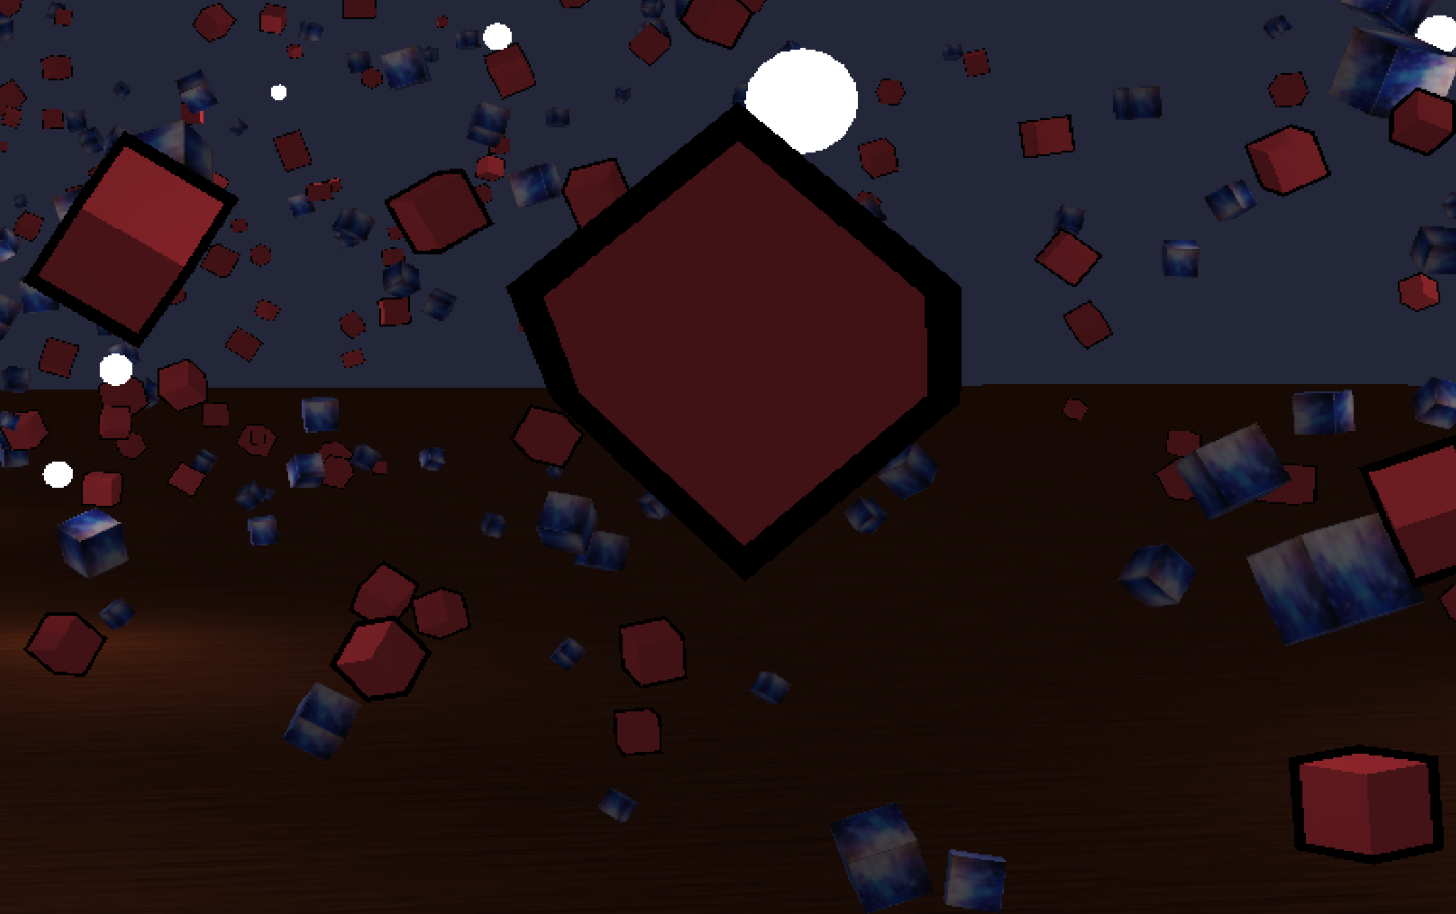
\includegraphics[width=\textwidth]{Abbildungen/IMG-20260711205352333}
        \caption{Inverted-Hull in Forward}
        \label{fig:hydra_inverted-hull}
    \end{subfigure}
    \hfill
    % Rechtes Bild
    \begin{subfigure}[b]{0.49\textwidth}
        \centering
        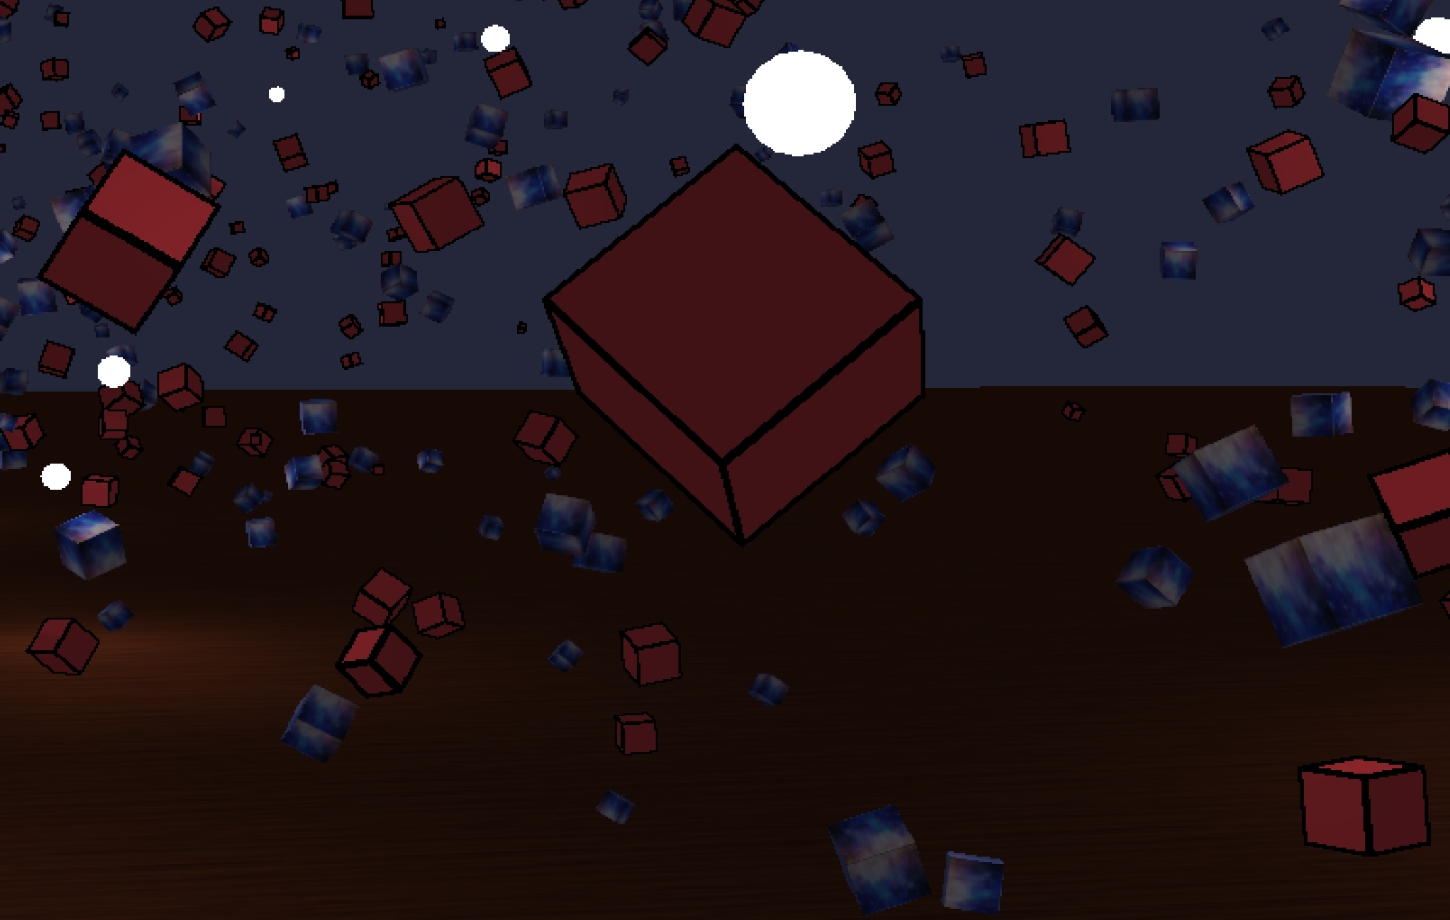
\includegraphics[width=\textwidth]{Abbildungen/IMG-20260711205459842}
        \caption{Sobel-Outlines in Deferred}
        \label{fig:hydra_solebl-outlines}
    \end{subfigure}
    \caption{Vergleich von Kontureffekten in Forward und Deferred mittels Inverted-Hull- und Sobel-Outline-Verfahren.}
    \label{fig:040201_outline_comparison}
\end{figure}


